\begin{center}
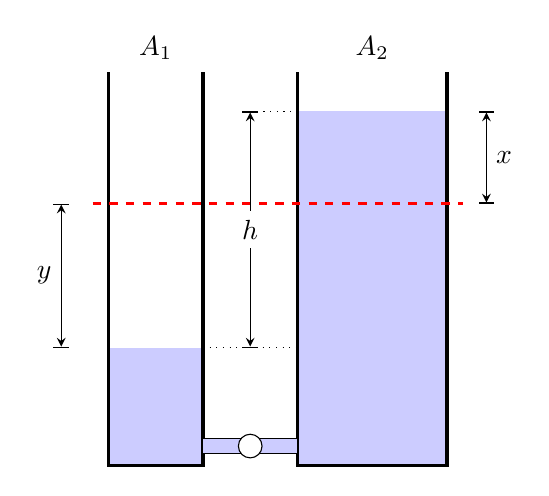
\begin{tikzpicture}[>=stealth]
 \fill[blue!20] (0,0) rectangle (1.2,1.5);
 \fill[blue!20] (2.4,0) rectangle (4.3,4.5);
 \draw[very thick] (0,5) -- (0,0) -- (1.2,0) -- (1.2,5);
 \draw[very thick] (2.4,5) -- (2.4,0) -- (4.3,0) -- (4.3,5);
 \fill[blue!20] (1.2,0.15) rectangle (2.4,0.35);
 \draw (1.2,0.15) -- (2.4,0.15);
 \draw (1.2,0.35) -- (2.4,0.35);
 \draw[fill=white] (1.8,0.25) circle (0.15);
 \node at (0.6,5.3) {$A_1$};
 \node at (3.35,5.3) {$A_2$};
 \draw[red, thick, dashed] (-0.2,3.33) -- (4.5,3.33);
 \draw[|<->|] (-0.6,1.5) -- (-0.6,3.33) node[midway, left] {$y$};
 \draw[|<->|] (4.8,3.33) -- (4.8,4.5) node[midway, right] {$x$};
 \draw[dotted] (1.2,1.5) -- (2.4,1.5);
 \draw[dotted] (1.8,4.5) -- (2.4,4.5);
 \draw[|<->|] (1.8,1.5) -- (1.8,4.5) node[midway, fill=white] {$h$};
\end{tikzpicture}
\end{center}

Nach dem Öffnen fliesst Wasser vom grossen in den kleinen Zylinder, bis die Spiegel gleich hoch sind (rot gestrichelt). Im grossen Zylinder ($A_2 = \AgO$) sinkt der Spiegel um $x$, im kleinen ($A_1 = \AkO$) steigt er um $y$. Zusammen müssen sie den Höhenunterschied $h = \hUO$ ausgleichen, und das Volumen, das den grossen Zylinder verlässt, kommt im kleinen an:
\begin{align}
 x + y &= h \\
 A_2\,x &= A_1\,y
\end{align}
Setzt man $y = h - x$ in die zweite Gleichung ein, erhält man
\begin{align}
 x &= \xgF \\
   &= \frac{\Ak}{\Ak+\Ag}\cdot\hU \\
   &= \xg \approx \result{\xgP{-2}{2}}
\end{align}
